\documentclass{article}\usepackage{graphicx, color}
%% maxwidth is the original width if it is less than linewidth
%% otherwise use linewidth (to make sure the graphics do not exceed the margin)
\makeatletter
\def\maxwidth{ %
  \ifdim\Gin@nat@width>\linewidth
    \linewidth
  \else
    \Gin@nat@width
  \fi
}
\makeatother

\definecolor{fgcolor}{rgb}{0.2, 0.2, 0.2}
\newcommand{\hlnumber}[1]{\textcolor[rgb]{0,0,0}{#1}}%
\newcommand{\hlfunctioncall}[1]{\textcolor[rgb]{0.501960784313725,0,0.329411764705882}{\textbf{#1}}}%
\newcommand{\hlstring}[1]{\textcolor[rgb]{0.6,0.6,1}{#1}}%
\newcommand{\hlkeyword}[1]{\textcolor[rgb]{0,0,0}{\textbf{#1}}}%
\newcommand{\hlargument}[1]{\textcolor[rgb]{0.690196078431373,0.250980392156863,0.0196078431372549}{#1}}%
\newcommand{\hlcomment}[1]{\textcolor[rgb]{0.180392156862745,0.6,0.341176470588235}{#1}}%
\newcommand{\hlroxygencomment}[1]{\textcolor[rgb]{0.43921568627451,0.47843137254902,0.701960784313725}{#1}}%
\newcommand{\hlformalargs}[1]{\textcolor[rgb]{0.690196078431373,0.250980392156863,0.0196078431372549}{#1}}%
\newcommand{\hleqformalargs}[1]{\textcolor[rgb]{0.690196078431373,0.250980392156863,0.0196078431372549}{#1}}%
\newcommand{\hlassignement}[1]{\textcolor[rgb]{0,0,0}{\textbf{#1}}}%
\newcommand{\hlpackage}[1]{\textcolor[rgb]{0.588235294117647,0.709803921568627,0.145098039215686}{#1}}%
\newcommand{\hlslot}[1]{\textit{#1}}%
\newcommand{\hlsymbol}[1]{\textcolor[rgb]{0,0,0}{#1}}%
\newcommand{\hlprompt}[1]{\textcolor[rgb]{0.2,0.2,0.2}{#1}}%

\usepackage{framed}
\makeatletter
\newenvironment{kframe}{%
 \def\at@end@of@kframe{}%
 \ifinner\ifhmode%
  \def\at@end@of@kframe{\end{minipage}}%
  \begin{minipage}{\columnwidth}%
 \fi\fi%
 \def\FrameCommand##1{\hskip\@totalleftmargin \hskip-\fboxsep
 \colorbox{shadecolor}{##1}\hskip-\fboxsep
     % There is no \\@totalrightmargin, so:
     \hskip-\linewidth \hskip-\@totalleftmargin \hskip\columnwidth}%
 \MakeFramed {\advance\hsize-\width
   \@totalleftmargin\z@ \linewidth\hsize
   \@setminipage}}%
 {\par\unskip\endMakeFramed%
 \at@end@of@kframe}
\makeatother

\definecolor{shadecolor}{rgb}{.97, .97, .97}
\definecolor{messagecolor}{rgb}{0, 0, 0}
\definecolor{warningcolor}{rgb}{1, 0, 1}
\definecolor{errorcolor}{rgb}{1, 0, 0}
\newenvironment{knitrout}{}{} % an empty environment to be redefined in TeX

\usepackage{alltt}
\IfFileExists{upquote.sty}{\usepackage{upquote}}{}

\begin{document}
%\SweaveOpts{concordance=TRUE, echo=FALSE}

\title{Optimal management of a stochastically varying population when policy adjustment is costly} 

%\titlerunning{Short form of title}        % if too long for running head

\author{Carl Boettiger    \\
       Michael Bode      \\
        James N. Sanchirico \\
Jacob LaRiviere \\
Alan M. Hastings\\
Paul R. Armsworth
}




\maketitle


\section{Introduction}



\begin{itemize}
  \item Ecosystem management frequently set in terms of policy of quotas. 
  \item Policy relatively static and costly to change
  \item Meanwhile, the natural world is variable
  \item Optimal solutions typically track these shocks, resulting in impractical management recommendations in face of policy costs
\end{itemize}

\emph{Develop a figure to insert here comparing quotas that were set to the stock size estimated at that time in the stock assessment for two different fish stocks. We choose the two stocks to highlight variation in how responsive management can be. Suggested halibut and bluefin tuna.}

Empirics suggest not always as responsive as Reed solution. Explore conditions under which that makes sense. Idea is that regulator’s objective sometimes may not be `raw' NPV, but rather NPV with some penalties on fast changes. Possible reasons: pure administrative transaction cost of changing policies (reaching agreement), fishermens' preferences for less variable quotas, processing plants' preferences for less variable quotas especially if tied into contracts for canning and so forth. But we do not know what functional form of any such policy adjustment costs takes and it will be a lot of work to estimate it. Here we explore several plausible candidate functional forms that each reflect different ways these policy adjustment costs could work. Would be good to know if differences between functional forms is particularly important.

\section{Methods}

 Fish population dynamics / state equation.  We will assume Beverton-Holt dynamics with multiplicative environmental noise
    \begin{equation} 
      N_{t+1} = Z_t \frac{A N_t}{1 + B N_t}, 
\label{eq:state_equation}
    \end{equation}
where $N_t$ the stock size, $Z_t$ gives the stochastic shocks, which we assume are lognormally distributed and $A$ and $B$ are positive constants. HARVESTING SHOULD APPEAR IN THIS EQUATION.

We assume managers set an annual quota for harvesting $h_t$ (the control variable) after observing the stock size that year $N_t$ (the state variable), but while still being uncertain about future environmental conditions and stock sizes. Through time, this gives a time path of management actions ${\bf h}=(h_1,h_2,\dots)$ that depend on the stock sizes that were observed (a state dependent control rule). 

We assume that managers choose annual quotas to maximize the expected net present value (NPV) of the fishery. We take as a base case the situation where there are no costs associated with policy adjustment and the managers' objective is
\begin{equation}
\max_{{\bf h}}\mathbf{ E} ( NPV_{0} )=\max_{{\bf h}} \sum_0^\infty \mathbf{E} \left( \displaystyle \frac{\Pi_0(N_t,h_t)}{(1+\delta)^{t+1}} \right)
\label{eq:objective}
\end{equation}
where $\mathbf{E}$ is the expectation operator, $\delta>0$ is the discount rate and $\Pi_0$ is the net revenue from operating the fishery in a given year. In this base case, we assume the annual net revenue from fishing is 
  \begin{equation} 
    \Pi_0(N_t,h_t) = p h_t -  c_0 E_t
\label{eq:annual_netrevenue}
  \end{equation}
  where $E_t$ represents
  fishing effort. We assume catch is proportional to stock size and effort expended fishing that year, $h_t=qE_tN_t$ and constant $q>0$ is the catchability coefficient. In Eqn.~\ref{eq:annual_netrevenue}, $p$ is the price per unit harvest and $c_0$ the cost of fishing and we assume $p>0$ and $c_0>0$.

Taken together this objective function (\ref{eq:objective}) and the state equation (\ref{eq:state_equation}) define a stochastic dynamic programming problem that we solve using backwards recursion via Bellman's equation. We denote the resulting state-dependent, optimal control as ${\bf h_0^*}$. PRESUMABLY YOU USED A FINITE TERMINAL TIME IN WHICH CASE WE NEED TO REVISE TO REFLECT HOW YOU HANDLED THAT.

\subsection*{Costs of policy adjustment}
We compare this base case to three alternative problem formulations, each reflecting different plausible functional forms that costs of policy adjustment could take. In each, we assume managers can adjust the quota set in the fishery $h_t$ in a given year and that any policy adjustment costs are associated with changes to this control variable. 

First we assume that policy adjustment costs are directly proportional to the magnitude of the change in policy being proposed, such that larger changes to annual harvesting quotas incur greater policy adjustment penalties. Specifically, we replace $\Pi_0$ in the $NPV_0$ equation with 
\begin{equation}
  \Pi_{1}(N_t,h_t, h_{t-1}) = \Pi_0 - c_1  |  h_t - h_{t-1} | \,.
\end{equation}

Next we continue to assume that policy adjustment costs depend on the magnitude of the change in policy being proposed. However, we consider a case where this dependence is nonlinear with big changes in policy being disproportionately expensive:
\begin{equation}
  \Pi_{2}(N_t,h_t, h_{t-1}) = \Pi_0 - c_2 (  h_t - h_{t-1})^2 \,.
\end{equation}

Finally, we assume instead that there is a fixed cost associated with any adjustment of policy, regardless of how large that adjustment might be
\begin{equation}
  \Pi_{3}(N_t,h_t, h_{t-1}) = \Pi_0 - c_3 (1-\mathbf{I}(h_t, h_{t-1}))  \,,
\end{equation}
where indicator function $\mathbf{I}(h_t, h_{t-1})$ takes the value 1 if $h_t=h_{t-1}$ and zero otherwise. For each $\Pi_i$, we can then define a new objective function $NPV_i$ similar to that in Eqn.~\ref{eq:objective}. 

Taken together with the state equation (Eqn.~\ref{eq:state_equation}), each of these new objective functions defines a different stochastic dynamic programming problem. Again, we solve them numerically using backwards recursion.  To include costs of policy adjustment, we expand the state space to include both the current stock size and the management action taken on the previous time step $(N_t,h_{t-1})$. For each new objective function $\max NPV_i$, we denote the corresponding optimal control policy $ {\bf h_i^*} $.

In addition in the Supplementary Material, we compare our results with a more conventional fisheries economic formulation in which additional costs are applied to the control variables themselves, as opposed to adjustments to the controls: $ \Pi_4 (N_t,h_t) = p h_t -  c_0 E_t-c_4E_t^2$. Additional costs of this form tend to have  a smoothing effect on optimal quotas, but also change the long-term average stock size or quota size that is optimal.

\subsection*{Choice of parameters}

Each of the policy adjustment cost function is characterized in terms
of a cost coefficient $c_i$.  However, $c_i$ takes different units for each  functional form. Therefore, if seeking to compare the relative effect of each penalty function on optimal management, it is unclear what parameter values should be used. To address this issue, we calibrate choices of $c_i$ so that each has a comparable impact on the optimal net present value of fishery, broadly following the example of Bovenberg, Goulder and Gurnery (2005) and Bovenberg, Goulder and Jacobsen (2008).

Figure 1 shows the calibration graphically.  Each curve plots the change in maximum expected NPV for a given penalty function as the penalty cost parameter is increased. In each case, the figure shows maximum expected NPV with policy adjustment costs as a proportion of the maximum expected NPV available in the basic problem $NPV_0({\bf h_0^*})$ without policy adjustment costs. 

To compare the impact of penalty functions on optimal management across the different functional forms, we select penalty cost coefficients that induce the same reduction in maximum expected NPV. For example, the dashed vertical lines in Figure 1 map the needed cost coefficient $c_i$, for each penalty function, such that the fishery is worth 80\% of its unconstrained value when optimally managed. 

Other parameters in the model are chosen - HOW? 






\begin{figure}
\begin{knitrout}
\definecolor{shadecolor}{rgb}{0.969, 0.969, 0.969}\color{fgcolor}
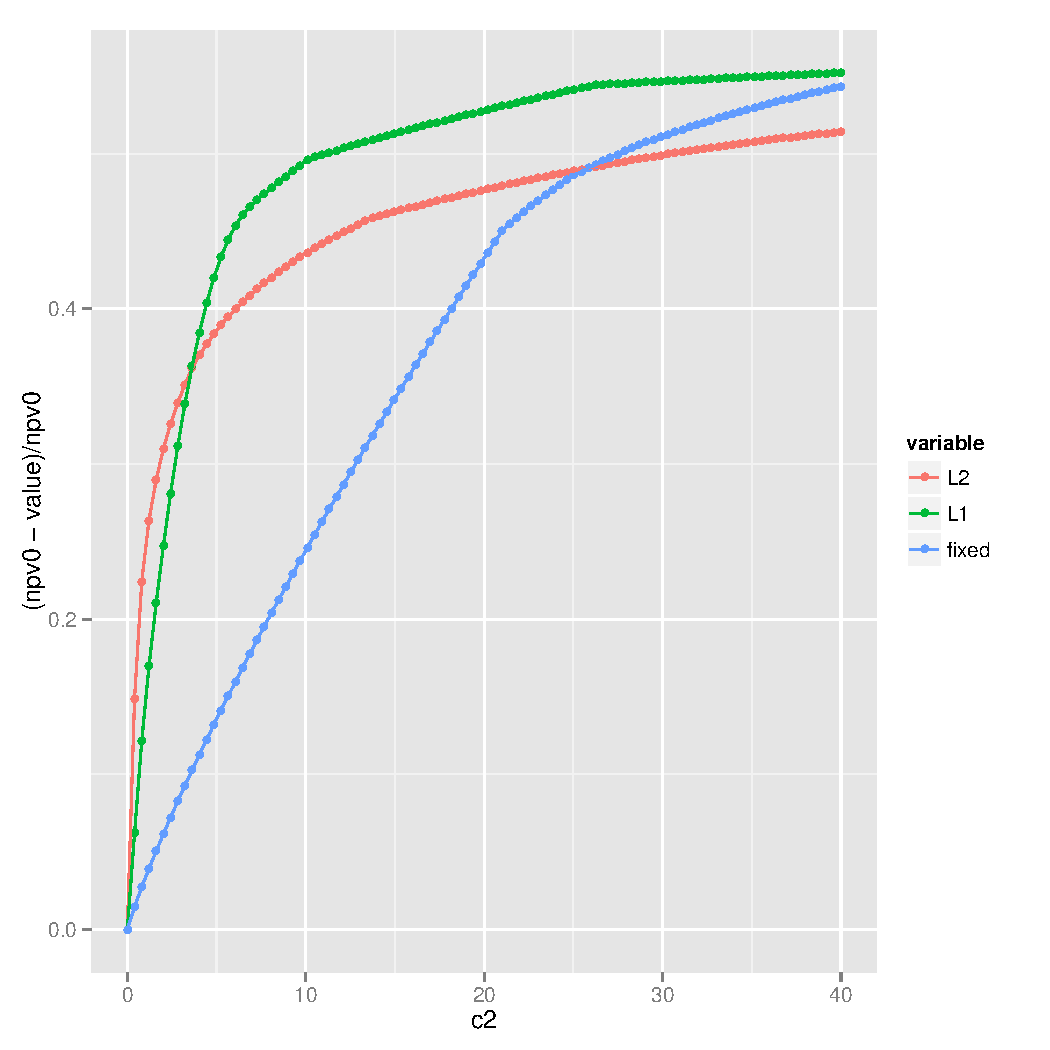
\includegraphics[width=\maxwidth]{figure/Figure_1} 

\end{knitrout}


\caption{\textbf{Expected net present value by functional form of penalty.} Horizontal axis shows the coefficient $c_i$ governing the magnitude of the policy cost, while vertical axis shows fraction of the maximum expected net present value dissipated by the policy cost.  The horizontal line indicates a value of the stock that is 80\% of the maximum expected value in the absence of policy adjustment costs, $NPV_0({\bf h_0^*})$. Selecting the coefficient $c_i$ corresponding to this value in each functional form allows us to make consistent comparisons across the different functional forms of policy costs.  }
\end{figure}

\section{Results}
\subsection*{Effect of policy adjustment costs on optimal quotas and stock sizes}
Figure 2 shows the impact that the adjustment cost has on the optimal policy.   Each panel is generated against the same sequence of random shocks so that they can be compared directly. Figure 3 (TO COME) shows the corresponding stock sizes.  In each case, the optimal solution without any adjustment cost is shown in black and the policy induced by optimization under the given adjustment penalty (equivalent to a 25\% reduction in maximum expected NPV) is overlaid in blue.  

When considering the first formulation of policy adjustment costs ($\Pi_1$), the first  panel of Figure 2 shows a typical pattern, in which the optimal policy tends to avoid small policy adjustments, resulting in long periods of constant policy followed by sudden bursts of adjustment. This results in a relatively step-like policy pattern.  In contrast, the second formulation $\Pi_2$ disproportionately penalizes large policy adjustments. The corresponding optimal policy tracks all of the changes made by the cost-free policy, but with smaller magnitude.  This results in a smoother $h_t$ curve, one that undershoots the larger oscillations seen in the cost-free optimum in favor of a policy that changes incrementally each yearl.  Finally, the optimal policy for the third, `fixed fee' formulation ($\Pi_3$) only makes large adjustments, as one might expect, because the magnitude of the adjustment made is not reflected in the resulting penalty.  Whereas the optimal solution for $\Pi_1$ attempts to accommodate the large oscillations at the end of the period shown (time steps $t=47-49$) with a constant quota in between the extremes, the fixed fee version takes the opposite approach of one very large swing. MORE DETAILING TO COME WHEN WE HAVE THE FIGURES

\begin{figure}
\begin{knitrout}
\definecolor{shadecolor}{rgb}{0.969, 0.969, 0.969}\color{fgcolor}
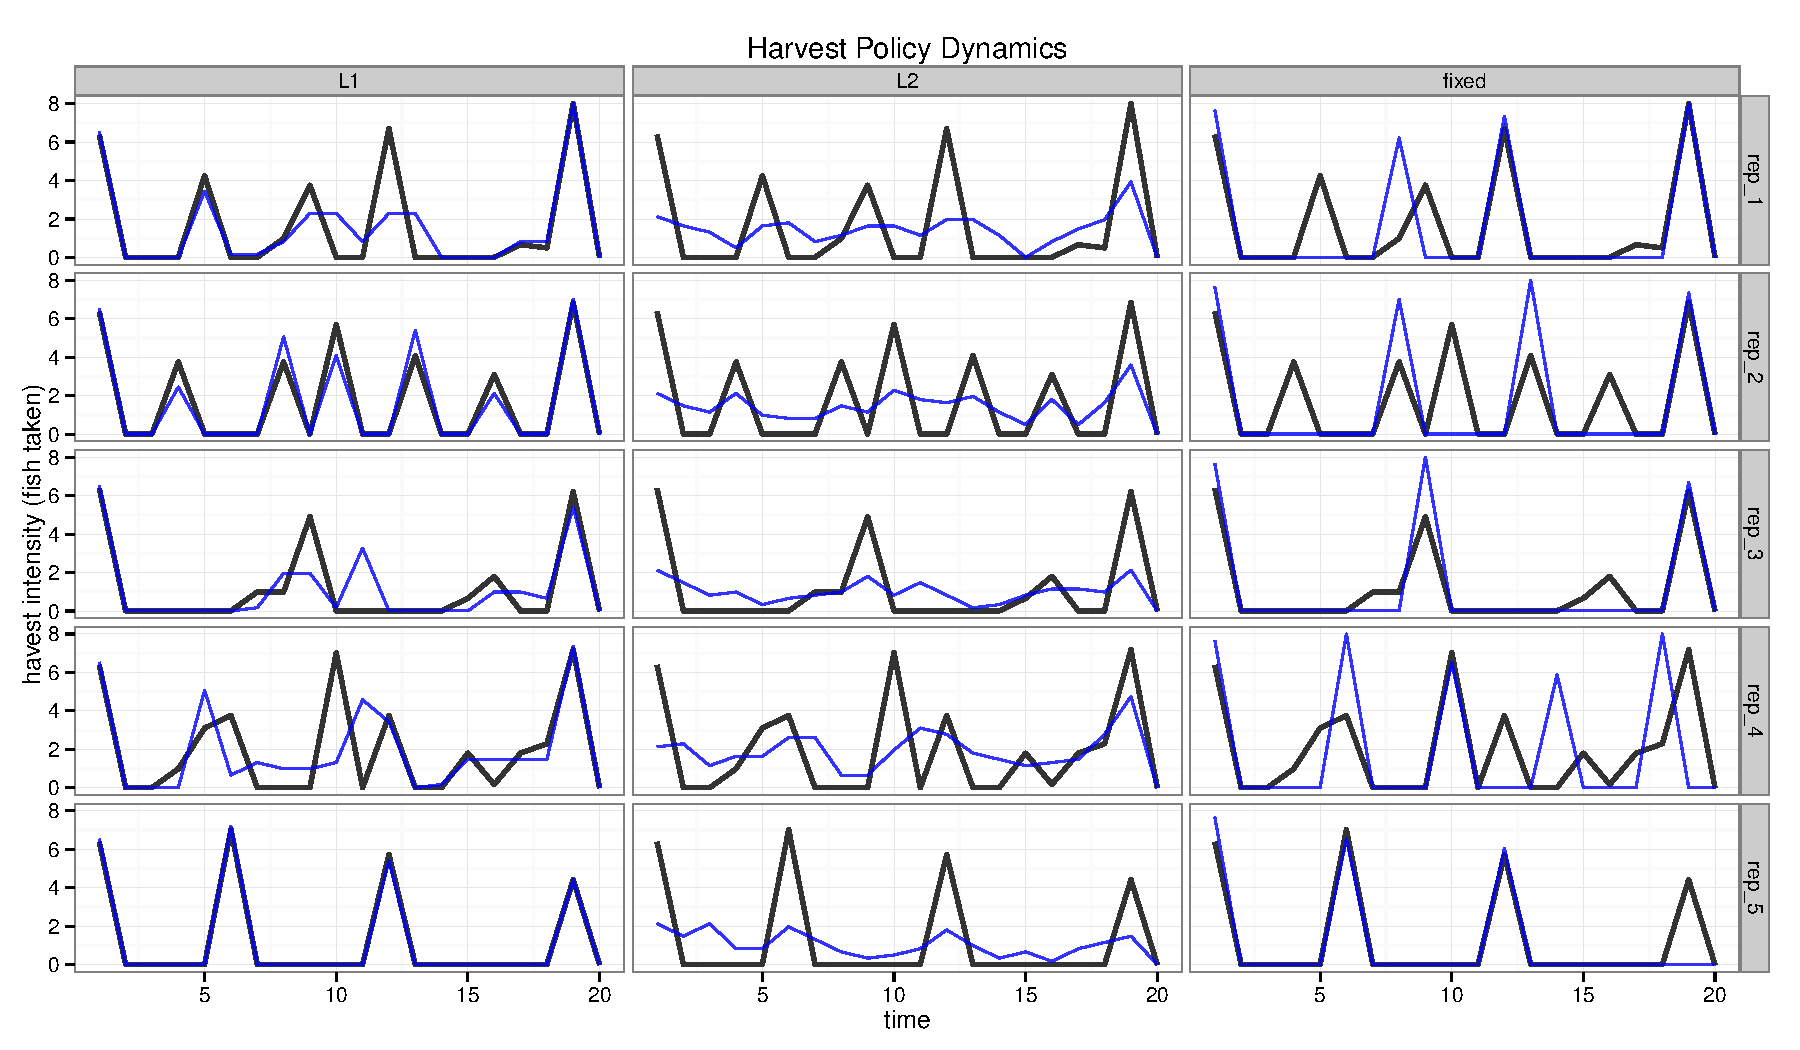
\includegraphics[width=\maxwidth]{figure/Figure_2} 

\end{knitrout}

  \caption{Individual realizations of optimal harvesting strategy under the different functional forms of adjustment costs.}
\end{figure}


\begin{figure}
\begin{knitrout}
\definecolor{shadecolor}{rgb}{0.969, 0.969, 0.969}\color{fgcolor}
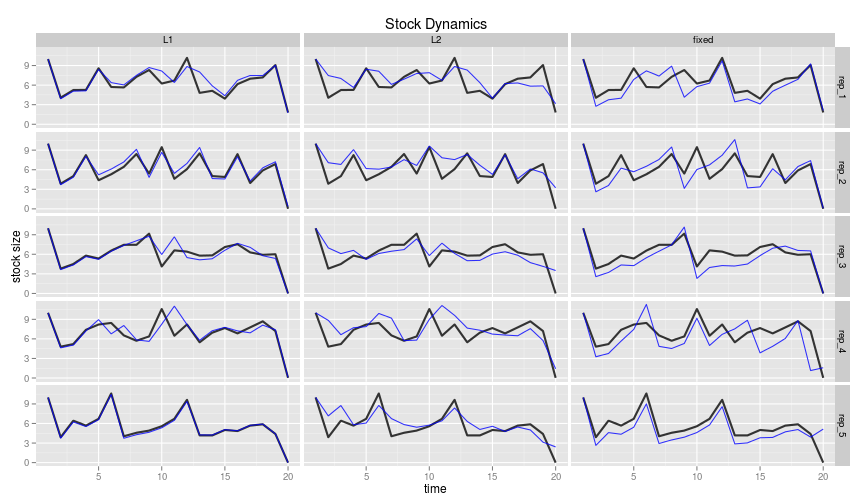
\includegraphics[width=\maxwidth]{figure/Figure_3} 

\end{knitrout}

  \caption{Individual realizations of optimal stock size strategy under the different functional forms of adjustment costs.}
\end{figure}



The comparisons shown in Figure 2 are for one realization (i.e. a particular sequence of random number draws representing environmental variability) and are made for a particular magnitude of policy adjustment costs equal to 25\% of the maximum expected net present value in the base case ($NPV_0({\bf h_0^*})$). Figure 4 generalizes to show how optimal harvest levels and corresponding optimal stock sizes are affected by the magnitude of the costs of policy adjustment. This time we show summary statistics across 50 replicate sets of environmental conditions. We show the impact of policy adjustment costs on the variance of both harvests and stock sizes through time; on the autocorrelation of harvests and stock sizes through time; and on the cross-correlation of harvests and stock sizes through time.  (COMPARABLE FIGURES FOR OPTIMAL STOCK SIZES AND CROSS-CORRELATIONS OF THE TWO TO COME.)

We see that TO COME WHEN WE HAVE THE FIGURES

\begin{figure}
\begin{knitrout}
\definecolor{shadecolor}{rgb}{0.969, 0.969, 0.969}\color{fgcolor}
\includegraphics[width=\maxwidth]{figure/Figure_4a} 

\end{knitrout}


\caption*{Figure 4a: Variance of optimal harvest rates through time as a function of size of adjustment penalties, the latter being calculated as percentage of the maximum expected NPV in the basic case with no policy adjustment costs. }
\end{figure}

\begin{figure}
\begin{knitrout}
\definecolor{shadecolor}{rgb}{0.969, 0.969, 0.969}\color{fgcolor}
\includegraphics[width=\maxwidth]{figure/Figure_4b} 

\end{knitrout}

\caption*{Figure 4b: Autocorrelation of optimal harvest rates through time as a function of size of adjustment penalties, the latter being calculated as percentage of the maximum expected NPV in the basic case with no policy adjustment costs. }
\end{figure}





\begin{figure}
\begin{knitrout}
\definecolor{shadecolor}{rgb}{0.969, 0.969, 0.969}\color{fgcolor}
\includegraphics[width=\maxwidth]{figure/Figure_5a} 

\end{knitrout}


\caption*{Figure 5a: Variance of optimal stock sizes through time as a function of size of adjustment penalties, the latter being calculated as percentage of the maximum expected NPV in the basic case with no policy adjustment costs. }
\end{figure}

\begin{figure}
\begin{knitrout}
\definecolor{shadecolor}{rgb}{0.969, 0.969, 0.969}\color{fgcolor}
\includegraphics[width=\maxwidth]{figure/Figure_5b} 

\end{knitrout}

\caption*{Figure 5b: Autocorrelation of optimal stock sizes through time as a function of size of adjustment penalties, the latter being calculated as percentage of the maximum expected NPV in the basic case with no policy adjustment costs. }
\end{figure}









\subsection*{Consequences of policy adjustment costs}

Next we examine the consequences either of ignoring policy adjustment costs when they are present or assuming they are present when they are not. To do so, it helps to break-down the different contributions to the maximum expected $NPV_i$ when employing the optimal policy $\bf{h_i}^*$ versus when employing the policy that would be optimal were there no costs to policy adjustment $\bf{h_0}^*$. For example, if we take the first of the adjustment penalty forms, $\Pi_1$
\begin{equation}
 NPV_i( \mathbf{h_1^*} ) = \sum_{t=0}^\infty (\overbrace{ p h^*_{1,t}-c_0E^*_{1t}}^{[1]}-\overbrace{c_1 | h^*_{1,t}- h^*_{1,t-1}|}^{[2]} ) \displaystyle \frac{1}{(1+\delta)^t}
\end{equation}
and 
\begin{equation}
 NPV_i( \mathbf{h_0^*} ) = \sum_{t=0}^\infty (\underbrace{ p h^*_{0,t}-c_0E^*_{0t}}_{[3]}-\underbrace{c_1 | h^*_{0,t}- h^*_{0,t-1}|}_{[4]} ) \displaystyle \frac{1}{(1+\delta)^t}
\end{equation}

Histograms for the different contributions labelled $[1]-[4]$ here when taken across XXX replicate runs are shown are shown in Figure 5 (contribution $[1]$ red, $[2]$ green, $[3]$ blue, and $[4]$ mauve). The cost of assuming policy adjustments are present when in fact they are absent is given by subtracting the contribution to the first infinite sum from term $[1]$ from the contribution to the second infinite sum of term $[3]$ (red-blue in the Figure). (Note that convergence properties required to do this are met because we assume a positive discount rate). This cost is positive because the optimal controls recommended when assuming policy adjustment costs are present do not track variations in stock size as closely. Therefore, this harvesting strategy provides lower net revenue dockside.

In contrast, the cost of ignoring policy adjustment costs when in fact they are present is given by subtracting the second infinite sum from the first (contributions $([1]-[2])-([3]-[4]))$ in the equations. These costs are positive because the lost revenues from not tracking stock variations as closely are smaller than the penalties of policy adjustment that are incurred if managers try to track stock variations more tightly.

\begin{figure}
\begin{knitrout}
\definecolor{shadecolor}{rgb}{0.969, 0.969, 0.969}\color{fgcolor}\begin{kframe}


{\ttfamily\noindent\itshape\color{messagecolor}{\#\# Using\ \ as id variables}}\end{kframe}
\includegraphics[width=\maxwidth]{figure/Figure_6} 

\end{knitrout}


\caption{Ignoring the cost of policy adjustment results in greater profits from fishing, but even greater costs for adjusting the harvest quotas each year.}
\end{figure}


\begin{figure}
\begin{knitrout}
\definecolor{shadecolor}{rgb}{0.969, 0.969, 0.969}\color{fgcolor}
\includegraphics[width=\maxwidth]{figure/Figure_7} 

\end{knitrout}

\end{figure}




Table 1 compares these different contributions, namely the $NPV$ lost by assuming policy adjustment costs when none are present (first entry in each cell, $[1]-[3]$ in the equations)) and the $NPV$ lost when ignoring policy adjustment costs when they are present (second entry in each cell of the table, contributions $([1]-[2])-([3]-[4]))$ in the equations) across the three different functional forms. Specifically, the table shows how these values change as we vary the severity of policy adjustment costs and the underlying environmental variability. In each case, values are shown as percentages of the maximum expected $NPV$ in the base case where no policy adjustment costs apply or are assumed to apply $NPV_0({\bf h_0^*})$.


% latex table generated in R 3.0.2 by xtable 1.7-1 package
% Wed Nov  6 20:50:41 2013
\begin{table}[ht]
\centering
\begin{tabular}{rlrrrrrr}
  \hline
 & penalty\_fn & ignore\_cost & ignore\_fraction & assume\_cost & assume\_fraction & sigma\_g & reduction \\ 
  \hline
1 & L1 & 14536.09 & 1.00 & 16857.61 & 1.00 & 0.05 & 0.10 \\ 
  2 & L2 & 11020.10 & 0.76 & 15538.44 & 0.92 & 0.05 & 0.10 \\ 
  3 & fixed & 13584.97 & 0.92 & 17582.78 & 1.05 & 0.05 & 0.10 \\ 
  4 & L1 & 9273.66 & 1.09 & 17561.81 & 1.04 & 0.05 & 0.20 \\ 
  5 & L2 & 11020.10 & 0.76 & 15538.44 & 0.92 & 0.05 & 0.20 \\ 
  6 & fixed & 8332.45 & 0.84 & 17401.82 & 1.03 & 0.05 & 0.20 \\ 
  7 & L1 & -641.78 & 0.21 & 15451.25 & 0.92 & 0.05 & 0.30 \\ 
  8 & L2 & -272586.11 & -24.90 & 11567.12 & 0.69 & 0.05 & 0.30 \\ 
  9 & fixed & -1213.01 & -0.46 & 15519.95 & 0.92 & 0.05 & 0.30 \\ 
  10 & L1 & 18281.97 & 1.01 & 20973.56 & 0.99 & 0.20 & 0.10 \\ 
  11 & L2 & 12462.51 & 0.72 & 19392.85 & 0.91 & 0.20 & 0.10 \\ 
  12 & fixed & 16691.94 & 1.03 & 20143.80 & 0.95 & 0.20 & 0.10 \\ 
  13 & L1 & 12788.95 & 0.96 & 20663.21 & 0.97 & 0.20 & 0.20 \\ 
  14 & L2 & 12462.51 & 0.72 & 19392.85 & 0.91 & 0.20 & 0.20 \\ 
  15 & fixed & 12399.01 & 0.88 & 21289.21 & 1.00 & 0.20 & 0.20 \\ 
  16 & L1 & 9099.48 & 0.73 & 19999.07 & 0.94 & 0.20 & 0.30 \\ 
  17 & L2 & -6337.76 & -0.39 & 17765.33 & 0.83 & 0.20 & 0.30 \\ 
  18 & fixed & 7399.01 & 0.62 & 21969.84 & 1.03 & 0.20 & 0.30 \\ 
  19 & L1 & 30227.43 & 1.07 & 31377.07 & 0.94 & 0.50 & 0.10 \\ 
  20 & L2 & 33472.18 & 1.00 & 33472.18 & 1.00 & 0.50 & 0.10 \\ 
  21 & fixed & 28926.73 & 1.09 & 30500.85 & 0.91 & 0.50 & 0.10 \\ 
  22 & L1 & 24157.93 & 1.10 & 31767.92 & 0.95 & 0.50 & 0.20 \\ 
  23 & L2 & 19091.31 & 0.93 & 29225.46 & 0.87 & 0.50 & 0.20 \\ 
  24 & fixed & 23573.19 & 1.02 & 30069.80 & 0.90 & 0.50 & 0.20 \\ 
  25 & L1 & 21086.12 & 1.12 & 32035.93 & 0.96 & 0.50 & 0.30 \\ 
  26 & L2 & 19091.31 & 0.93 & 29225.46 & 0.87 & 0.50 & 0.30 \\ 
  27 & fixed & 17209.56 & 0.85 & 32946.24 & 0.98 & 0.50 & 0.30 \\ 
   \hline
\end{tabular}
\end{table}




Overall cost of assuming policy adjustment costs apply when they are absent (first value) or from ignoring them when they are present (second value). These overall costs are shown for different severities of policy adjustment costs (columns) and levels of environmental variability (rows) and for three different functional forms for policy adjustment costs ($\Pi_i$ for $ i=1-3$). Values expressed as percentages of the maximum expected net present value when no policy adjustment costs apply and this is known to managers ($ NPV_0 ({\bf h_0^*}) $). 


MORE DETAILING WHEN WE HAVE THE TABLE.

\section{Discussion}
TO COME PENDING WHAT THE RESULTS SHOW.
\begin{itemize}
\item From Meeting 3: Interest in how the inclusion of these costs would operationally put a population at greater risk of extinction (e.g. if including the transaction costs increases the variance and autocorrelation of $N$ when subject to the optimal policy). Should expect this, because as the transaction costs become infinite, you would never change your policy which puts you in the world of open loop control - TAC fixed for all time, which we know puts the stock at greater risk of extinction.
\item On Table 1 should flag that might also be good to look at autocorrelated environmental noise and how that affects thing. Here we look at how the optimal policy induces more color in the stock size EVEN though the environmental variability going into it is white noise. - QUERY - HOW MUCH AUTOCORRELATION INDUCED BY STOCK DYNAMICS IN THE ABSENCE OF HARVESTING
\item for case of bluefin, interpreting  (1), (2), (3), and (4) in terms of how much you would have available to pay the Japanese and Canadians to convince them to participate in an expedited process to change TACs. Similarly for other contexts.
\item   Comparison of the optimal policy solution to the Reed model, traditional economic smoothing penalty - which now appears in SI
\item  Comparison between the different functional forms -- smoothing (L2)
  non-smoothing (L1), and de-stablizing (fixed).
\item   Induced costs (relative to free adjustment) vs direct costs (paid for adjusting) 
\item   Contrast steady-state results to dynamic solutions under stochastic shocks.
\end{itemize}

\textbf{Key conclusions:}
\begin{enumerate}
  \item \textbf{Lesson for modelers}: Ignoring the reality of policy costs leads to less effective management (decreased value)  (increased extinction risk?)
  \item \textbf{Lesson for policy makers}: Decreasing adjustment costs not only saves direct costs, but permits higher-value solutions.
\end{enumerate}





\end{document}
